In generale, il sistema consiste in una rete \textit{Peer-To-Peer} (\textbf{P2P}) che utilizza \textit{Proof-of-Work} (\textbf{POW}) per registrare l'elenco delle transazioni in un archivio pubblico, detto \textbf{blockchain}. Per una migliore comprensione del fenomeno si rimanda alla lettura dell'articolo originale di Satoshi Nakamoto \href{https://bitcoin.org/bitcoin.pdf}{Bitcoin}. 
L'implementazione del progetto è, almeno in parte, ripresa da quella descritta nell'articolo, fatta eccezione per lo sviluppodella Proof-of-Work, che segue i principi della criptovaluta \href{http://primecoin.io/bin/primecoin-paper.pdf}{\textbf{Primecoin}}.

In questa sezione sono enunciate le definizioni di transazioni (contenute in un blocco) e blockchain, e se ne discute la relativa implementazione. Sono poi elencate le definizioni delle altre componenti del sistema: il meccanismo di convalida di un blocco (la Proof-of-Work); il server Timestamp per la sincronizzazione oraria; il comportamento della rete all'avvio dell'esecuzione.

\subsection{Le transazioni e la catena di blocchi: la Blockchain}
La \textbf{blockchain} è una struttura dati ordinata, una lista concatenata di blocchi contenenti transazioni. L'intera struttura della blockchain può essere conservata in un file, oppure in un database. Un \textbf{block}, o blocco, è un contenitore, una struttura dati a sua volta, che aggrega transazioni che devono essere incluse in un \textit{ledger}\footnote{Il termine ledger indica il libro mastro dei contabili, viene tradotto in italiano come registro.} pubblico e condiviso, la blockchain. 
Il blocco è composto da un \textit{header}, che contiene i \textit{metadata}, e dalla lista di transazioni che ne compongono la maggior parte della grandezza.

\subsubsection{Implementazione}
\begin{enumerate}
    \item L'ID del blocco;
    \item Il hash del blocco precedente;
    \item Lunghezza della Proof-of-Work;
    \item Il numero primo origine (descritto più avanti);
    \item La catena di numeri primi che compone la Proof-of-Work di quel blocco;
\end{enumerate}

\subsection{Il Server Timestamp}
Un server timestamp offre un servizio che permette di conoscere l'ora esatta all'interno della rete. Un nodo che intende effettuare le operazioni di scrittura o di validazione di un blocco deve richiedere il \textbf{timestamp} al server. Esso garantisce l'esistenza dei dati al momento della richiesta.

\subsubsection{Implementazione}
In particolare, Jolie offre, tramite l'interfaccia \texttt{time} una \texttt{operation} che restituisce i millisecondi del \textit{current unix timestamp} nel momento esatto della richiesta. Tramite una chiamata a tale servizio si può ottenere il dato necessario da includere nel blocco. Qui è riportato un esempio si chiamata a tale operation, che può essere inserita in un server che accetta richieste e le inoltra al servizio time.
%
\lstinputlisting[language=Jolie]{code/timestamp.ol}
%

\subsection{La Proof-of-Work}
La Proof-of-Work, è un algoritmo che viene utilizzato per raggiungere un accordo decentralizzato tra diversi nodi nel processo di aggiunta di un blocco specifico alla blockchain.
Tale algoritmo produce valori che vengono utilizzati per verificare che sia stata eseguita una notevole quantità di lavoro. Nell'immagine riportata qui sotto viene visualizzato un esempio di utilizzo di tecniche Proof-of-Work nel mondo delle criptovalute (in particolare quella di Ethereum ma generalizzabile a qualunque altra che usa Proof-of-Work).
Per implementare un sistema decentralizzato basato su rete P2P, abbiamo bisogno di usare un sistema di Proof-of-Work\footnote{\url{http://www.wisdom.weizmann.ac.il/~naor/PAPERS/pvp.ps}}. Questo metodo consiste nell'obbligare i nodi che vogliono scrivere un blocco a cercare un valore che sia difficile da trovare e di cui sia facile controllarne la correttezza da parte degli altri nodi che vogliono validare la scrittura.
\begin{center}
    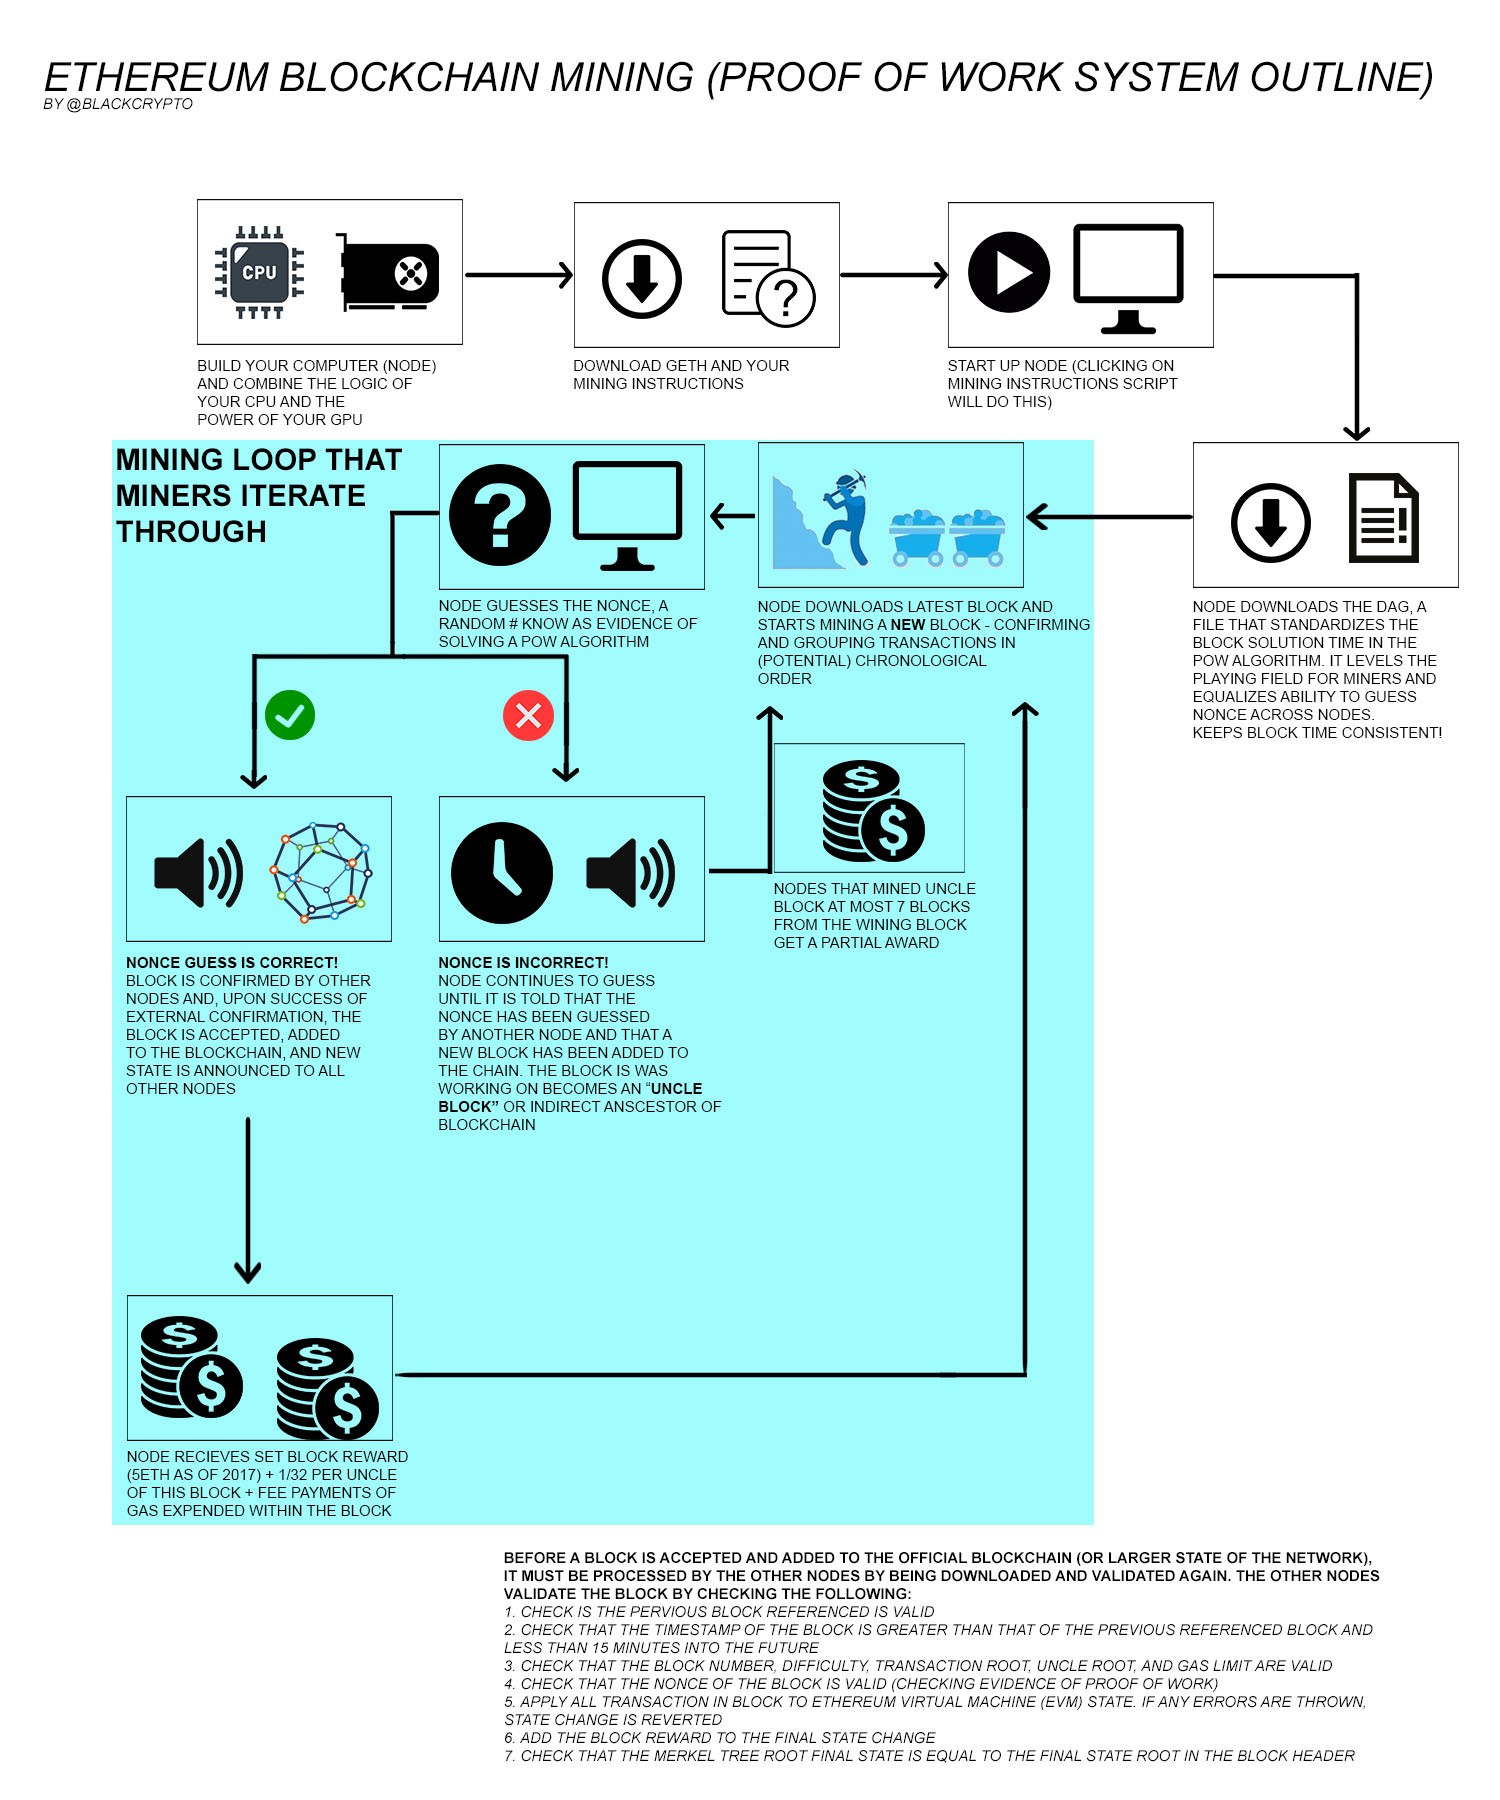
\includegraphics[width=\linewidth]{img/pow}
\end{center}

\subsubsection{Implementazione}
La Proof-of-Work scelta per produrre blocchi ed ottenere così sei Jollar in \textit{reward}\footnote{A differenza di Bitcoin, il reward in questo caso è fissato a sei ed è costante per tutta la vita della rete, un \textit{improvement} possibile è cambiare questo valore in una funzione decrescente.} è quella utilizzata dalla moneta PrimeCoin. Essa consiste nel generare delle catena di numeri primi con determinate proprietà.

\subsubsection*{Catene di Cunningham del Primo Tipo}
Una catena di Cunningham del primo tipo di lunghezza $k$ è un array di numeri primi:
\begin{center}
    $n-1,2n-1,\dots,2^{k-1}n-1$
\end{center}
Il numero $n$ è chiamato l'\textbf{origine} della catena. L'origine di una catena va va incluso nel blocco! Un esempio:
\begin{itemize}
    \item origine: $n=5$
    \item lunghezza: $k=5$
    \item catena: $2,5,11,23,47$
\end{itemize}

\subsubsection*{Catene di Cunningham del Secondo Tipo}
Una catena di Cunningham del secondo tipo di lunghezza $k$ è un array di numeri primi:
\begin{center}
    $n-1,n+1,2n-1,2m+1,\dots,\dots,2^{k-1}n-1,2^{k-1}n+1$
\end{center}
Un esempio:
\begin{itemize}
    \item origine: $n=4$
    \item lunghezza: $2k=4(k=2)$
    \item catena: $5,7,11,13$
\end{itemize}

\subsubsection*{Catene Bi-twin}
Una catena di Bi-twin di lunghezza $2k$ è una catena di $k$ numeri primi
\begin{center}
    $n-1,2n-1,\dots,2^{k-1}n-1$
\end{center}
 Un esempio:
\begin{itemize}
    \item origine: $n=5$
    \item lunghezza: $k=5$
    \item catena: $5,7,11,13$
\end{itemize}
Le catene Bi-twin posso anche essere viste come l'unione di due catene di Cunningham del primo o del secondo tipo con la stessa origine e lunghezza.
%
\subsection*{Validazione delle catene}
Il meccanismo di controllo e validazione delle Proof-of-Work inviate contenenti le catene di numeri primi prevede un test che utilizza il piccolo Teorema di Fermat (\href{http://primes.utm.edu/notes/proofs/FermatsLittleTheorem.html}{link alla dimostrazione}), esso afferma che, per $p$ primo ed $a$ intero 
\begin{center}
$a^{p-1} \equiv 1 (\bmod p)$ se $p$ non divide $a$.
\end{center}

\noindent I $p$ che soddisfano questo proprietà vengono chiamati \textit{pseudoprimi}, perché non tutti sono appunto primi. Vale però che maggiore è $p$, maggiore è la probabilità che sia primo. 

\noindent Un esempio utilizza tipicamente $a=2$ e lo eleva alla $p-1$ (prendiamo $17$ e $23$) che modulo p risulta essere uguale ad $1$:
\begin{center}
$2^{16}= 65536 \bmod 17 = 1$ \\
oppure \\
$2^{22}= 4194304 \bmod 23 = 1$
\end{center}

Ciò significa che per la primalità va controllata per ogni numero primo della catena. Inoltre la validazione controlla anche che la lunghezza della catena sia maggiore o uguale alla difficoltà (quindi il tipo di catena va incluso nel blocco!)

\subsection{La Rete Peer-To-Peer}
Una rete P2P, come ad esempio quella di \href{www.emule-project.net/home/perl/}{Emule}, è una rete i cui nodi non sono \textbf{client} o \textbf{server} fissi, ma prendono forma di entità equivalenti o ``paritarie''.
\begin{center}
    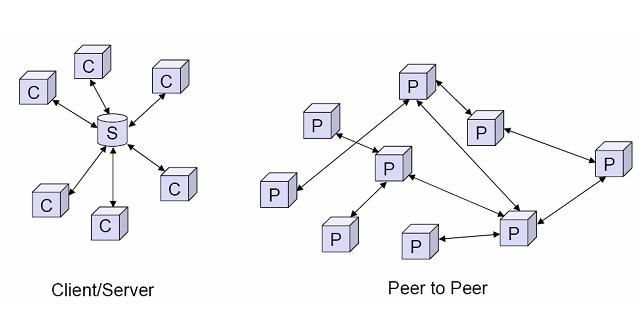
\includegraphics[width=\linewidth]{img/p2p}
\end{center}

\subsubsection{Implementazione}
L'esecuzione della rete P2P comprende i seguenti passaggi:
\begin{enumerate}
    \item Le nuove transazioni sono inviate in \textit{broadcast}\footnote{Nelle reti di calcolatori, il termine broadcast indica una modalità di instradamento per la quale un pacchetto dati inviato ad un indirizzo particolare (detto appunto di broadcast) verrà consegnato a tutti i computer collegati alla rete} a tutti i nodi che partecipano alla rete;
    \item Ogni nodo colleziona la nuove transazione in un blocco (una transazione per blocco!);
    \item Ogni nodo effettua del ``lavoro'' per provare di poter scrivere il blocco (Proof-of-Work);
    \item Quando un nodo trova una prova, invia il blocco in broadcast a tutti i nodi;
    \item I nodi accettano il nuovo blocco solo se la transazione contenuta in esso è valida e non è stata già ``spesa'';
\end{enumerate}

I nodi considerano sempre la blockchain più lunga come quella corretta. Nel caso in cui due nodi inviano versioni differenti del nuovo blocco contemporaneamente, alcuni nodi potrebbero riceverne  una versione, altri l'altra. In quel caso il nodo lavora sul blocco ricevuto temporalmente prima. Il nodo che ha lavorato su un blocco non sincronizzato se ne rende conto quando una nuova validazione viene richiesta, in questo caso egli manda in broadcast una richiesta di sincronizzazione sul blocco in questione e, una volta ricevuta risposta, aggiorna la blockchain alla versione più recente, potendo così validare il nuovo blocco ricevuto.

\subsection{Il Network Visualiser}
Il Network Visualiser è un tool amministrativo da terminale per il monitoraggio del sistema.

\subsubsection{Implementazione}
Il Network Visualizer invia richieste a tutta la rete per conoscere lo stato delle blockchain di tutti i nodi, la loro versione, le transazioni che contengono, generando le seguenti informazioni:
\begin{itemize}
    \item La data e l'ora del server timestamp al momento della richiesta.
    \item Per ogni utente/nodo: la sua chiave pubblica; le transazioni che ha effettuato divise per entrate/uscite; la versione della blockchain che utilizza e la quantità totale di Jollar che possiede.
    \item Per ogni transazione al punto precedente, ordinate in ordine cronologico, si indica la data, l'ora, e gli utenti (con le loro chiavi pubbliche) coinvolti.
    \item La blockchain più lunga presente nella rete (chiamata la versione ufficiale), con tutta la struttura dati che contiene.
\end{itemize}